\documentclass{sig-alternate}

%% anglicky jazyk dokumentu, vyuzite vsade v dokumente
\usepackage[english]{babel}
%% uprava ako su zobrazovane cisla stran, tiez uprauje styly nad ramec standardnych layoutov
%% vyuzite v hlavice dokumentu
\usepackage{fancyhdr}

\pagestyle{fancy}
\fancyhf{}
\rhead{UMAP’17, July 9-12, 2017, Bratislava, Slovakia}
\lhead{PALE: Personalization Approaches in Learning Environments}
\renewcommand{\headrulewidth}{0pt}
\newcommand\blfootnote[1]{%
  \begingroup
  \renewcommand\thefootnote{}\footnote{#1}%
  \renewcommand{\footnotesize}{\scriptsize}
  \addtocounter{footnote}{-1}%
  \endgroup
}
\renewcommand{\footnotesize}{\scriptsize}
\newcommand\tab[1][1cm]{\hspace*{#1}}

%% zlepsuje kvalitu tabuliek, pridava extra komandy a behind-the-scene optimalizaciu
%% vyuzite vo vsetkych tabulkach dokumentu
\usepackage{booktabs}

\pagenumbering{roman}

%% Balík stavia na grafickom balíku a poskytuje rozhranie kľúč - hodnota pre voliteľné argumenty pre príkaz \ includegraphics. Toto rozhranie poskytuje zariadenia, ktoré idú ďaleko nad rámec toho, čo ponúka grafický balík sám o sebe.
\usepackage{graphicx}

%% Balík prekladá rôzne štandardné a iné vstupné kódovania do „vnútorného jazyka LATEX“. Interný jazyk je vyjadrený výlučne v základnom kódovaní TEXu (štandardné ASCII tlačiteľné znaky, tokeny ovládania vozíka a kontrolné sekvencie TEX, ktoré sú väčšinou definované LATEXom).
\usepackage[utf8]{inputenc}

%% Hlavný balík v distribúcii AMS-LATEX. Prispôsobuje na použitie v LATEXe väčšinu matematických funkcií nájdených v AMS-TEX; vysoko sa odporúča ako doplnok k vážnemu matematickému sadzbe v LATEXu.
\usepackage{amsmath}

%% Štandardný LATEX bude prepínať iba medzi \ onecolumn a \ twocolumn v hornej časti stránky; samotné príkazy vymažú predchádzajúcu stránku. Tento balík odstraňuje obmedzenia a umožňuje kombinovať režimy jedného a dvoch stĺpcov na tej istej stránke.
%% vyuzite pri vlozeni obrazku cez oba stlpce stranky
\usepackage{cuted}% for environment `strip`

%% Ak sú umiestnené v texte bez toho, aby boli zapuzdrené v plávajúcom prostredí, môžu sa algoritmické prostredia rozdeliť na hranice stránky, čo značne znižuje ich vzhľad. Okrem toho je užitočné mať algoritmy očíslované pre referenciu a pre zoznamy algoritmov, ktoré sa majú pripojiť k zoznamu obsahu. Prostredie algoritmu je určené na riešenie týchto problémov poskytnutím plávajúceho prostredia pre algoritmy.
\usepackage{algorithm}
\usepackage[noend]{algpseudocode}
\makeatletter
\def\BState{\State\hskip-\ALG@thistlm}
\makeatother

%% Algorithm2e je prostredie na písanie algoritmov. Algoritmus sa stane plávajúcim objektom (napríklad obrázok, tabuľka atď.). Balík obsahuje makra, ktoré vám umožňujú vytvárať rôzne kľúčové slová, a poskytuje sa sada preddefinovaných kľúčových slov; môžete zmeniť typografiu kľúčových slov. Balík umožňuje zvislé čiary vymedzujúce blok inštrukcií v algoritme a definuje rôzne druhy algoritmov, ako napríklad procedúra alebo funkcia; názov týchto funkcií sa môže opätovne použiť v texte alebo v iných algoritmoch.
\usepackage[ruled,vlined,linesnumbered]{algorithm2e}
\usepackage{comment}

\begin{document}

\setlength{\heavyrulewidth}{1.2pt}
\setlength{\lightrulewidth}{0.7pt}

%% nadpis stranky
\title{Education-specific Tag Recommendation in CQA Systems}

%% autori
\numberofauthors{2}

\author{
\alignauthor
Peter Babinec\\
       \affaddr{Slovak University of Technology}\\
       \affaddr{Bratislava, Slovakia 841 04}\\
       \email{babinec.peter@gmail.com}\\
\alignauthor
Ivan Srba\\
       \affaddr{Slovak University of Technology}\\
       \affaddr{Bratislava, Slovakia 841 04}\\
       \email{ivan.srba@stuba.sk
}
}

\maketitle

%% zaciatok abstratu
\begin{abstract}
Systems for Community Question Answering (CQA) are well-known
on the open web (e.g. Stack Overflow or Quora). They have been
recently adopted also for use in educational domain (mostly in
MOOCs) to mediate communication between students and teachers.
As students are only novices in topics they learn about, they may
need various scaffolding's to achieve effective question answering.
In this work, we focus specifically on automatic recommendation
of tags classifying students’ questions. We propose a novel method
that can automatically analyze a text of a question and suggest appropriate tags to an asker. the method takes specifics of educational
domain into consideration by a two-step recommendation process
in which tags reflecting course structure are recommended at first
and consequently supplemented with additional related tags. Evaluation of the method on data from CS50 MOOC at Stack Exchange
platform showed that the proposed method achieved higher performance in comparison with a baseline method (tag recommendation
without taking educational specifics into account).
\end{abstract}

%% zaciatok CCS konceptov
\begin{CCSXML}
    <ccs2012>
    
    <concept>
    <concept_id>02</concept_id>
    <concept_desc>Computing methodologies~Virtual reality</concept_desc>
    <concept_significance>300</concept_significance>
    </concept>
    
    <concept>
    <concept_id>01</concept_id>
    <concept_desc>Information systems~Recommended system~ Question answering</concept_desc>
    <concept_significance>500</concept_significance>
    </concept>
    
    <concept>
    <concept_id>03</concept_id>
    <concept_desc>Appliedcomputing~E-learning</concept_desc>
    <concept_significance>200</concept_significance>
    </concept>
    
    </ccs2012>
\end{CCSXML}

\ccsdesc[500]{Information systems~Recommended systems;\textit{ Qu\\estion answering}}
\ccsdesc[300]{Human-centered computing~Social tagging}
\ccsdesc[200]{Appliedcomputing~E-learning}

\printccsdesc

%% klucove slova
\keywords{tag recommendation, community question answering, MO\\OC}

%% prva sekcia
\section{Introduction}
	Massive Open Online Courses (MOOCs) brought a significant change to domain of Technologically-Enhanced Learning (TEL). While traditional TEL approaches tackle with relatively small groups of students (usually at a classroom level), typical MOOCs involve large online communities consisting of thousands of students coming
from around the whole world. 
\blfootnote{Permission to make digital or hard copies of all or part of this work for personal or classroom use is granted without fee provided that copies are not made or distributed for profit or commercial advantage and that copies bear this notice. Copyrights for components of this work owned by others than the author(s) must be honored. Request permissions from permissions @acm.org. UMAP’17 Adjunct, July 09-12, 2017, Bratislava, Slovakia ©2017 Copyright held by the owner/author(s).DOI:10.1145/3099023.3099081} 
%% blind footnote zobrazena v lavo dole na stranke	
    This shit had to be reflected in many concepts and processes including presentation of learning materials, assignments review
or communication between students and teachers. 
	Particularly communication became a significant issue since teaching a large number of students may result into many questions
and some more text related to various aspects of a course. Without appropriate computer-mediated support, instructors would be overloaded by students’ requests as
well as students would face great information overload. the most of MOOC platforms (e.g. edX\footnote{https://www.edx.org/}, Coursera\footnote{https://www.coursera.org/}) use standard discussion forums to facilitate communication. On the one hand, these forums are quite easy to use, on the other hand they provide only limited possibilities how to structure and organize their content. Typically discussion posts are assigned only to categories representing individual parts of a course. Following the specific needs of MOOCs, some instructors started
to use alternative external tools, such as social networking sites,
real-time challeng rooms or recently Community question Answering (CQA) systems [1]. In this work we focus particularly on CQA systems, e.g. Stack Overflow\footnote{http://stackoverflow.com/} or quora\footnote{https://www.quora.com/}%% odkazy pod ciarou
, which are well-known and successful examples of how collective intelligence can be harnessed on the open web. CQA systems provide a possibility to all members of their communities to ask a question as well as provide answers/comments on questions asked by the rest of the community (see our previous survey [16] for an overview of research tasks addressed in CQA systems). their many advantages already motivated researchers to examine their potential in educational domain, what resulted into several kinds of educational CQA systems. At first, there are large-scale open CQA systems (e.g. OpenStudy [13]), that involve students without any particular restriction on MOOC
or university. On the opposite side, there are CQA systems for students from a particular course (e.g. Piazza\footnote{https://piazza.com/} or Green Dolphin [2]). In our previous work, we introduced a novel concept of organizational CQA system Askalot [15]. Askalot involves students from the whole university and thus it allows a better flow of knowledge
from students in higher years to their younger peers. In contrast to standard discussion forums, CQA systems provide a more structured way of communication with better content organization - particularly tags are mostly used. Tags, created either
individually or collaboratively (so called folksonomy), can serve users for search, navigation or awareness of new content (e.g. users in educational CQA system Askalot get notifications about new questions assigned with tags they watch [15]). In addition, tags may be utilized as a source of meta description, which can be further
used for user/domain modeling, personalization or recommendation. In our previous work, we recognized social tagging in the educational system ALEF [5] as a powerful tool for domain model building from the bottom up.

	In contrast to CQA systems on the open web, educational CQA
systems are characterized by many specifics. Among them, students
may have significant troubles to select appropriate tags during the
process of question creation. This problem is even more eminent in
educational CQA systems as in non-educational ones, since students
are only novices in course topics and thus they may be unfamiliar
with domain terms. In addition, students may not be aware of
importance of tag selection. This can be illustrated on Askalot CQA
system, which was used at Quantum Cryptography course (with
about 9 200 enrolled students) in MOOC system edX. In this course,
tag selection was only optional during question creation. Only 125
out of 508 questions (24.61)
Following this motivation, we can witness in educational CQA
systems a compelling need to support students during tag selection.
It can be done by tag recommendation. In this paper, we present
a novel approach for tag recommendation proposed specifically
for questions in educational CQA systems. According to our best
knowledge, this is the first approach which tackles with tag recom-
mendation specifically designed for educational CQA systems.
This paper is organized as follows. Section 2 reviews state-of-the-
art approaches to tag recommendation in context of CQA systems
and TEL. Section 3 describes a dataset obtained from a selected
educational CQA system. Section 4 introduces our method for tag
recommendation. Section 5 presents on experimental evaluation.

%% druha sekcia
\section{RELATED WORK}
Tag recommendation is a specific kind of well-known document
classification task which aims to assign a document into one or
more categories. Documents may be represented by a text, images,
videos or other kinds of multimedia. In our work, we tackle par-
ticularly with textual documents - questions (consisting of title
and description) and tags at the place of categories that questions
should be assigned to.
On the basis of state-of-the-art literature review, we recognized
that tag recommendation can be approached very miscellaneously.

%% cislovany zoznam
\begin{enumerate}
\item At first, research on tag recommendation can be divided
into graph-based and content-based approaches [10]. In
the first group, a graph representing users, documents and
tags is created (e.g. adaptive probabilistic hypergraph [11]).
Afterwards, various graph-based metrics are used to iden-
tify similar questions or related tags candidates. The main
limitation of graph-based methods is sparsity of the graphs
[10]. This problem can be addressed by content-based ap-
proaches, which focus primarily on the document content,
and thus they can recommend tags also for documents
with only limited information in the graph.
\item  Secondly, tag recommendation methods differ in \\ information they exploit. The previous works utilize mainly [4]: 1)
terms extracted from multiple textual features; 2) term/tag
co-occurrence; and 3) tag relevance. Additional data are
less commonly utilized, such as user-document-tag rela-
tionship or users’ tag usage history.
\item Some approaches may consider pre-assigned tags, for ex-
ample to infer tag co-occurrence information (e.g. [4]).
While other methods work without any information about
previously assigned tags (e.g. [10]).
\item Finally, another distinction lies in the scope of tags that
methods can suggest to a document. While the majority of
approaches work with a set of existing tags, few approaches
(e.g. [12]) can also suggest completely new tag candidates
by identification of keywords from a document.
\end{enumerate}

%% sekcia druhej urovne
\subsection{Tag Recommendation in Context of CQA
}
In the context of CQA systems, two main approaches to question
classification exist. At first, questions are organized by a hierarchy
of categories (e.g. in Yahoo! Answers). Secondly, questions are
organized by a set of tags (e.g. Stack Overflow or Quora). While a
notable research effort has been spent on category classification (e.g.
[3] or [6]), just a few approaches tackle with tag recommendation.
There is only one graph-based approach by [11], who proposed
an adaptive probabilistic hypergraph, in which hyperedges can be
constructed not only from a question content but also from question
answering history of an asker and his/her followees. The remaining
approaches can be characterized as content-based.
Nishida and Fujimura [12] proposed a hierarchical classification
method, in which a hierarchy of tags consists of three abstraction
levels: category, theme and keyword.
Saha et al. [14] introduced a discriminative model for suggesting
tags to Stack Overflow questions. It consists of three main steps:
1) converting questions into vectors (with term frequency weight-
ing scheme); 2) training a discriminative model (built with SVM
classificators); and finally 3) suggestion of tags with top similarity.
Xia et al. [17] proposed a tag recommendation method TagCom-
bine which was evaluated on Stack Overflow and Freecode datasets.
In contrast to the previous approaches, the proposed method com-
bined 3 components: 1) a multi-label ranking component which
considers tag recommendation as a multi-label learning problem;
2) a similarity based ranking component which recommends tags
from similar objects; 3) a tag-term based ranking component which
considers the relationship between different terms and tags.

%% sekcia
\section{DATASET DESCRIPTION
}
In this paper, we proceed from a dataset from educational CQA
system CS50 at Stack Exchange platform\footnote{https://cs50.stackexchange.com/} . This CQA system was
created primarily for students enrolled in CS50 edX course\footnote{https://www.edx.org/course/introduction-computer-science-harvardx-cs50x} pro-
vided by Harvard University.
It is an introductory course explaining basics of computer science,
such as algorithms, data structures, software engineering and web development. Students solve various tasks assigned to 9 problem
sets and one final project. Several languages are used by students
including C, Python, SQL, JavaScript or HTML.
Our dataset was obtained via Stack Exchange API and covers
questions posted between May 2014 and February 2017. It consists
of 6365 questions and 796 tags. The more detailed statistics about
the dataset are depicted in Table 1. We found out that about 66.4%
of all questions contain a code snippet. It means that various code
constructions present a potential to predict tags corresponding to
various programming languages.
When we analyzed a long-tail distribution of tag usage (see
Figure 1), we found out that among the most frequent tags many
correspond to problem sets (designated as pset0 to pset8) or final
project (final-project). In total, even about 74% of all questions
have a tag referring to a related problem set (almost all of them
have exactly one of those tags). The similar categorical tags, which
express a relation between questions and parts of the course, are
present in the most of educational CQA systems (e.g. also in Piazza
or Askalot).
We also recognized that despite Stack Exchange mechanism for
tags deduplication (manually defined tag synonyms are used to
merge redundant tags with the same meaning), there are still some
undesirable duplicates. At the same time, we identified incorrectly
created tags that mostly join two individual tags, e.g. pset5-load.These inconsistencies had to be addressed in the proposal of our
method in order to achieve a truly high-quality tag prediction.

%% tabulka
\begin{table}[]
\caption {CS50: Statistical analysis of questions
}
%% volny riadok
\hfill \break
\begin{center}
\begin{tabular}{|l|l|l|l|l|}
\hline
\textbf{Name} & \textbf{Tags} & \textbf{Answers} & \textbf{Views} & \textbf{Score} \\ \hline
mean          & 2.40          & 1.14             & 206.26         & 0.26           \\ \hline
std           & 1.06          & 0.65             & 605.70         & 0.85           \\ \hline
minimum       & 1             & 0                & 4              & -7             \\ \hline
25\%          & 2             & 1                & 41             & 0              \\ \hline
50\%          & 2             & 1                & 80             & 0              \\ \hline
75\%          & 3             & 1                & 178            & 0              \\ \hline
maximum       & 5             & 8                & 20268          & 19             \\ \hline
\end{tabular}
\end{center}
\end{table}

%% vlozeny graf
\begin{figure}
  \centering
    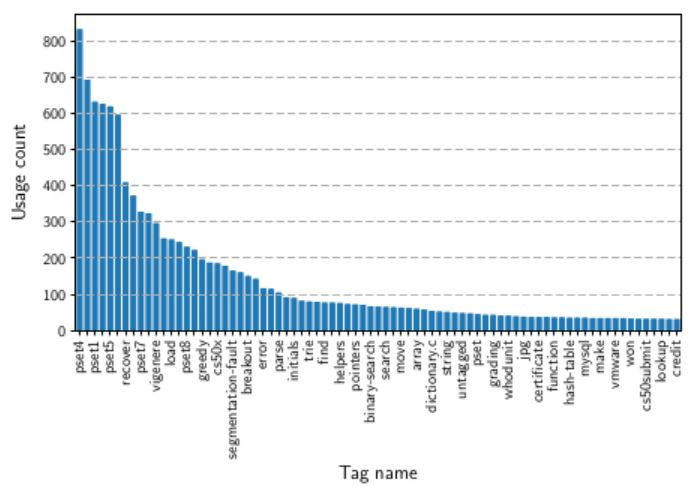
\includegraphics[width=\columnwidth]{graf01.JPG}
  \caption{Most frequent tag distribution.
}
  \label{fig:graph}
\end{figure}

%% sekcia
\section{TAG RECOMMENDATION METHOD \\ FOR
EDUCATIONAL CQA SYSTEMS}

In this section, we present an overall framework for tag recommen-
dation designed specifically for educational CQ A systems.
The proposed method belongs to the group of content-based tag
recommendation approaches. It is fundamentally based on terms
extracted from a title and a description of a question and it also
considers tag co-occurrence. The method works also in situations
when no pre-assign tags are available and thus it can be used in
three different scenarios:

%% cislovany zoznam
\begin{enumerate}
\item Primarily to recommend tags in real-time during question
creation process and thus supporting students with manual
tag selection.
\item To recommend additional tags for questions with incom-
plete set of existing tags.
\item To automatically identify incorrectly assigned tags.
\end{enumerate}
As we primarily intend to recommend tags for questions imme-
diately at their creation time, we cannot rely on additional infor-
mation from answers or comments. Finally, we restrict our method
on recommendation of existing tags only.
Our method is based on machine learning approach and consists
of four main phases that correspond to the stages in typical machine
learning workflow (see Figure 2).

%% podsekcia
\subsection{Data Preprocessing}
As we found out in Section 3, despite manual inspection (by sys-
tem moderators) and auto-correct mechanisms (by replacing tags
synonyms) the tags in CQA systems may be inconsistent. This
may negatively affect tag recommendation. Therefore, at first we
attempt to perform a tag correction. It can be done manually or
semi-automatically by definition of correction rules, however, in
both cases it is highly dependent on particular educational CQA
system and MOOC.
Besides tag correction, also questions themselves are prepro-
cessed. The content of each question (i.e. its title and description)
may be enriched with a formatting syntax (markdown). This may
negatively affect the following term extraction. So all formatting
marks are stripped while the intended code snippets are preserved.
The content is afterwards processed by standard NLP methods,
namely the text is tokenized and obtained words are lemmatized
and transformed to lowercase. Finally stop-words are removed.

%% podsekcia
\subsection{Feature Extraction and Transformation
}In the second phase, we convert preprocessed text of questions into
high-dimensional vectors, particularly into bag of words (BoW)
representation (based on unigrams). As a standard bag of words
model weights each term with a simple term frequency weight, we
apply a transformation to use a TF-IDF (term frequency - inverse
document frequency) weighting scheme instead, which represents
the term-document relevance more precisely.

%% podsekcia
\subsection{Model Training
}To estimate the appropriateness of a tag candidate to a question,
we utilize a supervised multi-label classification. Multi-label classi-
fication assigns a document (in our case a question) with a set of
labels (in our case a set of tags) which are not mutually exclusive.
The problem of multi-label classification is commonly addressed
by its transformation into a set of binary classification problems
(with one vs. rest strategy), which can be solved by standard binary
classification algorithms (e.g. SVM or Random Forest). Following
this approach also in our method, we train the model by training a
set of binary classifiers for each tag separately.

%% podsekcia
\subsection{Model Application and Evaluation
}In the last phase, we apply the trained model (the set of binary
classifiers) to predict the most suitable tag candidates. In this step,
we take into consideration the educational specifics that distinguish
standard CQA system from educational ones.
The main concept of our method is that we predict separately: 1)
categorical tags; and 2) related tags with taking their co-occurrence
with previously predicted categorical tags into account.
In the first step, we limit tag recommendation to categorical tags,
while the rationale for this decision is twofold. Firstly, presuming
that the course categories address different learning concepts, cate-
gorical tags are easier to predict, since the corresponding questions
are likely to use different terminology. Secondly, as the most of ques-
tions should be assigned with at least one categorical tag (except
general questions that do not tackle with a particular course part),
we explicitly consider their special role and minimize a number of
questions when categorical tags are missed.

%% vlozeny obrazok cez oba stlpce stranky
\begin{strip}
  \centering
  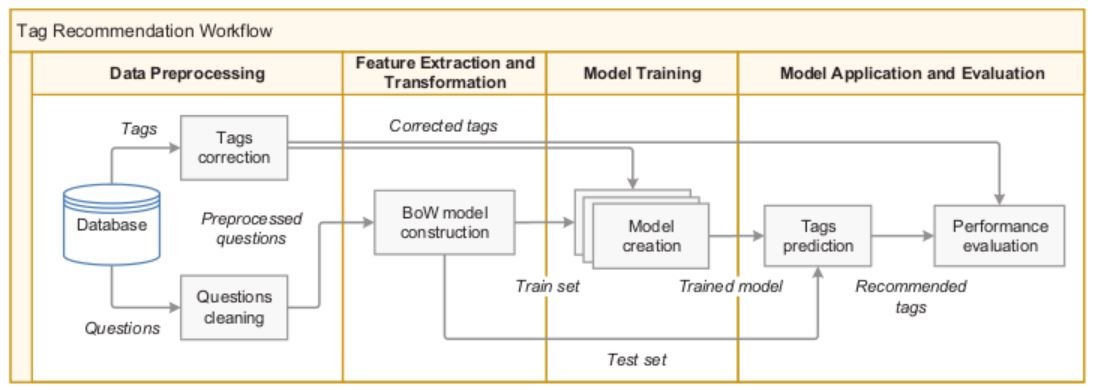
\includegraphics[width=\textwidth]{graf02.JPG}
  \caption{Figure 2: The phases of tag recommendation in the proposed method.}
  \label{fig:graph}
\end{strip}

%% pokracovanie textu podsekcie
Categorical tags can be easily distinguished from the remaining
tags (e.g. in the CS50 dataset, they have a standard naming conven-
tion pset{#n}; in Askalot system, categorical tags are predefined
by teachers and displayed differently). Nevertheless, there is still
an option to identify them automatically by considering their high
usage frequency and their close affinity with the learning domain
(e.g. number of their occurrence in learning materials).
In the second step, we supplement categorical tags with addi-
tional question-specific related tags. Similarly as in the previous
step, we apply each tag classifier on a question to get tag predic-
tions together with their predict probability (i.e. a classifier certaintythat the prediction is correct). These tags’ predict probabilities are
boosted by taking co-occurrence with the categorical tags (predicted
in the first step) into account (see Algorithm 1). For each categorical
tag, the new boosted predict probability Pnew is calculated as:

%% rovnica
\begin{equation*}
Pnew &= Pn + Pn * (1 - Pn) *\frac{count(Tn, CTx)}{max(count(T, CTx))}
\end{equation*}

%% pokracovanie textu podsekcie
where Pn is a previous value of predict probability; count (Tn , CTx )
is a number of co-occurrences of a related tag Tn and a categorical
tag CTx ; max(count(T , CTx )) is a maximal number of co-occurrences
between a categorical tag CTx and any tag T (used as a normaliza-
tion, which eliminates a popularity bias of the categorical tag).
The formula is derived to always keep Pnew within the range
< 0, 1 > and works well regardless the number of predicted cate-
gorical tags. Also in case of several categorical tags, boost never
significantly overcomes the previous probability Pn , since it de-
pends on Pn and its strength is decreasing slowly for already strong
Pn > 0.5. Maximal potential boost by 0.25 is achieved for the most
co-occurring tag and Pn = 0.5.
It would be possible to boost predict probability in the same
way also by co-occurrence with tags previously used by a student
(instead of categorical tags). It would make the tag recommendation
more personalized, nevertheless in educational domain, students
go through all course topics so their history do not reflect their
personal interests as it is in general CQA systems.
The final set of predicted tags is created by selecting predicted
categorical tags and supplementing them with the most probable
related tags (sorted by their boosted predict probabilities) so finally
top n tags are returned. In order to prevent recommendation of
tags with very low predict probability, the selection of relevant
tags should be limited by a threshold for minimal necessary predict
probability.

%% sekcia
\section{EXPERIMENTAL EVALUATION
}We evaluated our method in an offline experiment on the CS50
dataset from Stack Exchange platform described in Section 3.

%% podsekcia
\subsection{Experimental Setup
}We implemented our proposed method in Python programming lan-
guage. For machine learning and data manipulation the following
packages were used: scikit-learn, NumPy, SciPy and Pandas.

%% algoritmus
%% neslo mi vlozit jednu vertikalnu ciaru lebo program nespoznal pokyn "Predict Related Tag"
\begin{algorithm}[H]
\DontPrintSemicolon
\SetAlgoLined
\BlankLine
\SetKwInOut{Input}{Input}\SetKwInOut{Output}{Output}
\Input{categorical Predictions map of key-value pairs, keys
are questions and values are predicted categorical tags;
train Samples set for training containing questions
associated with all tags but categorical;
test Samples set for testing.
}
\Output{related Predictions map of key-value pairs, keys are
questions and values are predicted related tags.
}
\BlankLine

Predict Related Tag
\\(categorical Predictions, train Samples, test Samples)\
    \BlankLine
    model $M$ \longleftarrow  f it(trainSamples)
    \BlankLine
    relatedPredictions \longleftarrow  new Map(key, value)


\ForEach{question Q ∈ testSamples}{    
probabilities \longleftarrow M. predict Probabilities (Q)
categ\\orical Tags \longleftarrow categorical Predictions.get(Q)

    \BlankLine
    
    \ForEach{tag CT ∈ categorical Tags}{
    probabilities \longleftarrow boost(probabilities, CT )

      
                       
    }  
    related Tags\\
    decide(probabilities, count, threshold)\\
    relatedPredictions.add(Q, relatedT aдs)

}
\caption{Predicting related tags with boosting of predict
probabilities by co-occurrence with categorical tags.
}

\Return $relatedPredictions$

\end{algorithm}


%% pokracovanie textu
Tag correction was performed semi-automatically by definition
of correction rules describing which tags should be merged together
or on the contrary split into separate tags. Markdown from ques-
tions was removed by BeautifulSoup library. For performing NLP
tasks, NLTK library was used.
For experimental evaluation we selected only those tags that
have been assigned to at least 20 questions (what corresponds to
an average number of questions per tag). There are two motives for
this selection. At first, we prevent a possible cold start problem that
can cause an over-fitting for rare tags. Moreover, we want to rec-
ommend only those tags that are meaningful for search, navigation
or obtaining awareness of other classmates. After tag correction
and selection, we got 118 unique tags in total.
We divided the dataset into a train and test set chronologically
so the train set covers first two iterations of the course from 2014
to 2015 (4841 questions) and the test set covers the last iteration
of the course starting in 2016 (1302 questions). By this division,
we achieved an ecologically valid experiment as we simulated the
situation when the method is used across all problem sets.
Similarly as in the previous studies (e.g. [14], [17]), we consider
tags assigned by users as predicted labels. For performance evalua-
tion, we utilized standard metrics commonly used in information
retrieval and document classification, namely precision, recall and
F1 score. In addition, we evaluated a number of questions without
any tag recommendations (i.e. a number of cases when a method
cannot support an asker).
As the baseline, we used a tag recommendation method without
educational specifics (i.e. without two-step tag recommendation
and co-occurrence boosting of predict probability), which corre-
sponds to the approach proposed in [14]. This baseline recommends
all tags which are labelled with a positive class by their correspond-
ing binary classifiers and sorted by their predict probability.
In our method, we recommended categorical tags supplemented
with maximum of 3 related tags with the threshold for minimal
predict probability set at 0.5 (the threshold controls a trade-off
between precision and recall, therefore it is possible to set a higher
value to improve precision or a lower value to improve recall).

%% tabulka
\begin{table}[]
\caption {Comparison of the proposed method and baseline

}
\hfill \break
\begin{tabular}{|l|l|l|l|}
\hline
\textbf{Method used} & \textbf{Precision} & \textbf{Recall} & \textbf{F1 score} \\ \hline
Our method (SVM)     & 0.7038             & 0.5979          & 0.6465            \\ \hline
Baseline (SVM)       & 0.7003             & 0.5559          & 0.6198            \\ \hline
Our method (RF)      & 0.4708             & 0.6403          & 0.5426            \\ \hline
Baseline (RF)        & 0.6038             & 0.5717          & 0.5873            \\ \hline
\end{tabular}
\end{table}


%% podsekcia
\subsection{Results Description
}The design of our method allows us to use any binary classifier.
We selected particularly Support Vector Machines (SVM) and Ran-
dom Forest (RF) that achieved in the existing approaches the most
promising results. For both classifiers, we employed for a hyper-
parameter tuning a gridsearch to systematically explore the param-
eter space. Consequently, we applied a random search around the
best combination of parameters found by the gridsearch, what even
improved the performance of our as well as the baseline method.
In case of our method, the hyper-parameter tuning was done sep-
arately for prediction of categorical and related tags (the selected
parameters were different because in the case of related tags, the
classifiers need to tackle with a larger number of classes and a
bigger similarity between BoW models).
At first, we examined a performance of categorical tag recom-
mendation since its high precision is a prerequisite to successful
recommendation of related tags (in the case of incorrect categorical
tag assignment, incorrect tags would be boosted). SVM classifier
achieved precision at 92.87 and recall at 90.71, what sufficiently
satisfies our requirements.
Table 2 presents the comparison of overall performance (for cat-
egorical and related tags) achieved by the baseline method and our
proposed method. We can see a significantly better results for SVM
(in case of both methods), what confirms the conclusion from the
previous works that SVM is generally more successful for document
classification and high-dimensional vectors. While the precision
is approximately the same, we can see an improvement in recall
and F1 score of our education-specific method over the baseline
(our further analyses confirmed that the proposed co-occurrence
boosting leads to this improvement).
In addition, our method also significantly outperforms the base-
line in a number of questions with no predicted tags. Our further
analyses showed that the baseline failed to predict categorical tags
for 164 questions (14.7%), while our method only for 55 questions
(4.9%) out of 1112 questions that were actually assigned with at least
one categorical tag. It means that two-step recommendation, which
addresses categorical tags separately, actually helped to reduce a
number of cases, when important categorical tags are missed.

%% tabulka, nie vsetky udaje su prepisane doslova z povodneho dokumentu
\begin{table}[]
\caption{Table 3: Tag recommendations by the proposed method
}
\hfill \break
\label{tab:my-table}
\begin{tabular}{|l|l|l|l|}
\hline
\multicolumn{2}{|l|}{\textbf{User asigned}} & \multicolumn{2}{l|}{\textbf{Additionally predicted}} \\ \hline
\textbf{Matched}      & \textbf{Missed}     & \textbf{Correct}         & \textbf{Incorrect}        \\ \hline
Baseline (SVM)        &                     &                          &                           \\ \hline
Our method (RF)       & 0.4708              & load                     & 0.5426                    \\ \hline
pset2, vigenere       & 0.6038              & 0.5717                   & 0.5873                    \\ \hline
\end{tabular}
\end{table}

%% pokracovanie textu
%% aby sa percento zobrazilo v texte treba ho zapisat \%, necitala som cely dokument lebo je vedecky a po anglicky, tak asi miestami to chyba
As user-assigned tags may not be complete for some questions,
we conducted an additional posterior evaluation of tags recom-
mended by our method (with SVM predictors). We randomly se-
lected 100 questions (with 211 user-assigned tags in total) and for
each predicted tag, an expert annotator evaluated whether it is
correct for the corresponding question, incorrect or cannot decide.
Out of 173 predicted tags, 121 (70\%) matched user-assigned tags.
Out of 52 remaining predicted tags, 27 tags (52\%) were evaluated
by an annotator as correct. It confirms that our method can be
used also in the scenario when the recommended tags are used as
suggestions to complement the existing user-assigned tags.
To illustrate tags recommended by our method, we randomly
selected few examples that represent various cases of correct as
well as incorrect tag predictions (see Table 3).

%% sekcia
\section{DISCUSSION AND CONCLUSIONS
}
Tagging was previously recognized as essential and beneficial for
efficient learning, nevertheless there is a significant lack of research
addressing tag recommendation in educational domain. In this
paper, we proposed a novel method for tag recommendation specifi-
cally designed for educational CQA systems, that recently started to
appear as an alternative to standard discussion forums in MOOCs.
The novelty of our method lies in education-specific two-step
tag recommendation approach, in which we predict separately
important categorical tags (i.e. tags that are used to interconnect
the questions with particular parts of the MOOC). At the same time,
we are aware of some limitations of the proposed method in terms
of cold-start problem and robustness. In order to train the model
for existing tags, a sufficient number of previously correctly tagged
questions must exist. It means that the method is not applicable to
recommend very rare tags or at the beginning of the first iteration
of the course (when there are no previous questions). Secondly, the
course structure and learning materials can change in time (e.g. the
order of problem sets can change). These changes will naturally
influence the correctness of predicted tags, however, they will also
invalidate tags previously assigned to questions. So if these tags
will be readjusted to a new course structure, also all tag classifiers
can be retrained afterwards.
To evaluate the performance of our proposed method, we con-
ducted the offline experimental evaluation on the dataset from
CQA system CS50 at Stack Exchange platform. The results showed
that the proposed method achieved significantly better results in
comparison with the baseline. The precision of categorical tag rec-
ommendation was even about 93%. The overall precision and recall
of all tags was about 70% and 60% respectively. This performance im-
plies that we can provide students with reliable recommendation of
categorical tags and suggestions of top n additional related tags. In
addition, recommended tags can serve also as a source of metadata
for user modelling, content recommendation or personalization.

%% neocislovana sekcia
\setcounter{secnumdepth}{0} %% no numbering
\section{ACKNOWLEDGMENTS
}This work was partially supported by grants No. APVV-15-0508,
VG 1/0646/15, KEGA 028STU-4/2017 and it is the partial result of
collaboration within the SCOPES JRP/IP, No. 160480/2015.

%% bibliografia
\begin{thebibliography}{9}
\bibitem{} 
Carlos Alario-Hoyos, Mar Perez-Sanagustin, Carlos Delgado-Kloos, Hugo A.
Parada G., and Mario Munoz-Organero. 2014. Delving into Participants’ Profiles
and Use of Social Tools in MOOCs. IEEE Transactions on Learning Technologies 7,
3 (jul 2014), 260–266.
\bibitem{} 
Chulakorn Aritajati and N. Hari Narayanan. 2013. Facilitating Students’ Collab-
oration and Learning in a Question and Answer System. In Proceedings of the
2013 Conference on Computer Supported Cooperative Work Companion - CSCW
’13. ACM Press, New York, New York, USA, 101–106.
\bibitem{} 
Kyoungman Bae and Youngjoong Ko. 2012. An effective category classification
method based on a language model for question category recommendation
on a cQA service. In Proceedings of the 21st ACM International Conference on
Information and Knowle
\bibitem{} 
Fabiano Bel ́ m, Eder Martins, Tatiana Pontes, Jussara Almeida, and Marcos
e
Goncalves. 2011. Associative tag recommendation exploiting multiple textual
 ̧
features. In Proceedings of the 34th Int. ACM Conf. on Research and Development
in Information Retrieval - SIGIR ’11. ACM Press, New York, New York, USA, 1033.
%% konkretne prvky bibliografie
\bibitem{} 
M ́ ria Bielikov ́ , Mari ́ n Simko, Michal Barla, Jozef Tvaroˇ ek, Martin Labaj,
a
a
a ˇ
z
ˇ
R ́ bert M ́ ro, Ivan Srba, and Jakub Sevcech. 2014. ALEF: from Application to
o
o
Platform for Adaptive Collaborative Learning. In Recommender Systems for
Technology Enhanced Learning: Research Trends & Applications. Springer, Berlin,
Heidelberg, 195–225.

\bibitem{} 
Wen Chan, Weidong Yang, Jinhui Tang, Jintao Du, Xiangdong Zhou, and Wei
Wang. 2013. Community Question Topic Categorization via Hierarchical Ker-
nelized Classification. In Proceedings of the 22nd ACM International Conference
on Information and Knowledge management - CIKM ’13. ACM Press, New York,
New York, USA, 959–968.

\bibitem{} 
Ernesto Diaz-Aviles, Marco Fisichella, Ricardo Kawase, Wolfgang Nejdl, and
Avar ́ Stewart. 2011. Unsupervised Auto-tagging for Learning Object Enrichment.
e
Springer, Berlin, Heidelberg, 83–96.

\bibitem{} 
Simone Kopeinik, Elisabeth Lex, Paul Seitlinger, Dietrich Albert, and Tobias
Ley. 2017. Supporting collaborative learning with tag recommendations. In
Proceedings of the 7th International Learning Analytics & Knowledge Conference -
LAK ’17. ACM Press, New York, New York, USA, 409–418.

\bibitem{} 
Emanuel Lacic, Dominik Kowald, Paul Seitlinger, Christoph Trattner, and Denis
Parra. 2014. Recommending Items in Social Tagging Systems Using Tag and
Time Information. (jun 2014). arXiv:1406.7727

\bibitem{} 
Marek Lipczak and Evangelos Milios. 2010. Learning in efficient tag recom-
mendation. In Proceedings of the 4th ACM Conference on Recommender Systems -
RecSys ’10. ACM Press, New York, New York, USA, 167.

\bibitem{} 
Liqiang Nie, Yi-Liang Zhao, Xiangyu Wang, Jialie Shen, and Tat-seng Chua. 2014.
Learning to Recommend Descriptive Tags for Questions in Social Forums. ACM
Transactions on Information Systems 32, 1 (jan 2014), 1–23.

\bibitem{} 
Kyosuke Nishida and Ko Fujimura. 2010. Hierarchical Auto-Tagging: Organizing
Q&A Knowledge for Everyone. In Proceedings of the 19th ACM International
Conference on Information and Knowledge Management - CIKM ’10. ACM Press,
New York, New York, USA, 1657–1660.

\bibitem{} 
Ashwin Ram, Hua Ai, Preetha Ram, and Saurav Sahay. 2011. Open Social Learning
Communities. In Proceedings of the International Conference on Web Intelligence,
Mining and Semantics - WIMS’11. ACM Press, New York, New York, USA.

\bibitem{} 
Avigit K. Saha, Ripon K. Saha, and Kevin a. Schneider. 2013. A Discriminative
Model Approach for Suggesting Tags Automatically for Stack Overflow Ques-
tions. In Proceedings of 10th Working Conference on Mining Software Repositories -
MSR ’13. IEEE, 73–76.

\bibitem{} 
Ivan Srba and Maria Bielikova. 2015. Askalot: Community Question Answering
as a Means for Knowledge Sharing in an Educational Organization. In Proceedings
of the 18th ACM Conference Companion on Computer Supported Cooperative Work
- CSCW ’15 Companion. ACM Press, New York, New York, USA, 179–182.

\bibitem{} 
Ivan Srba and Maria Bielikova. 2016. A Comprehensive Survey and Classification
of Approaches for Community Question Answering. ACM Transactions on the
Web 10, 3 (aug 2016), 1–63.

\bibitem{} 
X Xia, D Lo, X Wang, and B Zhou. 2013. TagCombine: Tag Recommendation in
Software Information Sites.(2013). 10th Working Conference on Mining Software
(2013), 287–296.

\end{thebibliography}

\balancecolumns

\end{document}
